\documentclass{l4dc2026}
\usepackage{iftex,booktabs,longtable,array}
\ifPDFTeX
  \usepackage{times}
\else
  \usepackage{fontspec}
  \setmainfont{Times New Roman}
  \setmonofont{Courier New}
\fi
\jmlrvolume{}
\jmlrproceedings{ESE 6180}{ESE 6180 Experiment Analysis}
\jmlrworkshop{ESE 6180 Experiment Analysis}
\title[Pitfalls Experiment Analysis]{History, Coverage, and Action Chunking:\\Analysis of the Pitfalls Experiments}
\author{\Name{Nihar Ballamudi}\and\Name{Kyle Horton}\\\addr University of Pennsylvania}
\setlength{\emergencystretch}{1em}
\begin{document}
\maketitle
\begin{abstract}
We analyze eight retained experiment runs on the linear challenging example, separating effects of observation history, training coverage, and executed action chunks. Raw-rollout audits support the reported scores. Recovery training with two-step partial-observation history enables stable one-step execution, while narrow demonstrations remain underidentified. Longer history and longer execution can each help particular fitted controllers, but neither universally reduces tracking error. Archived noisy experiments, mean--median differences, long-run diagnostics, and initialization and distribution-shift limitations qualify these findings.
\end{abstract}
\section{What the pitfalls experiments actually show}
The experiments study whether a controller can recover from a departure that its demonstrations did not show, and whether history or action commitment can help. The strongest new result is conditional: with corrective training coverage, partial observation needs history two for accurate one-step control. Narrow data can remain inadequate even when the state is reconstructible.

\paragraph{History and training coverage solve different problems.}
History can make hidden state inferable. Recovery data teach how to act on it. Neither property alone guarantees a trained controller succeeds.

\paragraph{The original hard condition is narrow training.}
The expert stays on $x_1$=0, so the learner sees no expert correction to $x_1$. A small test departure exposes this missing behavior.

\paragraph{Long history is not always better.}
Narrow-data fits improve in the tested grid. With partial recovery training, history two is already sufficient and longer histories slightly increase tracking loss.

\paragraph{Stability and tracking are separate.}
A radius below one establishes eventual decay for the fitted linear loop. It does not establish accurate expert imitation. A small finite-rollout loss does not establish stability.

\paragraph{Scope of this review}
Eight saved runs are reviewed: five active snapshots and three archived versions. They contain 2,565 learned seed/configuration records, including repeated horizon prefixes and reused training seeds. This is not 2,565 independent experiments. No new controllers were trained for this report.

{\small The audit reconciled 1,215 controller-level means with 50,040 saved individual rollout rows, checked 2,400 serialized partial-observation inputs, and recorded hashes for 93 source files. Details and machine-readable values accompany the PDF.\par}

\section{Design: where the hardness enters}
The fixed plant is the two-dimensional linear component of the challenging pair in \citet{simchowitz2025}. At $\mu=1/8$, the matched expert makes $x_1$ vanish in one step and shrinks $x_2$ by 0.75 each step. The plant itself is also stable. A learned feedback controller can nevertheless destabilize it. In the paper, two plants share identical narrow demonstrations but need different off-support corrections. Our sweep fixes plant A1; it does not test the full two-plant worst-case guarantee.

\[x_{t+1}=Ax_t+u_t,\qquad u_t^\star=Kx_t.\]

{\small\setlength{\tabcolsep}{3pt}
\begin{longtable}{@{}p{\dimexpr 0.20833\linewidth-2\tabcolsep\relax}p{\dimexpr 0.38826\linewidth-2\tabcolsep\relax}p{\dimexpr 0.40341\linewidth-2\tabcolsep\relax}@{}}
\toprule
\textbf{Choice} & \textbf{What the learner receives} & \textbf{What the condition tests} \\
\midrule\endfirsthead
\toprule
\textbf{Choice} & \textbf{What the learner receives} & \textbf{What the condition tests} \\
\midrule\endhead
\bottomrule\endfoot
Full observation & Current/past $x_1$ and $x_2$, plus applied actions & Feedback selection with directly visible state \\
Partial observation & Only y=$x_2$, plus applied actions & Whether history resolves hidden $x_1$ \\
Narrow training & Expert trajectories confined to $x_1$=0 & Recovery behavior absent from training \\
Recovery training & Known-action exploratory histories with expert continuation labels & Learning with wider, informative coverage \\
\end{longtable}}

In recovery training, applied actions are Kx plus Gaussian probes of standard deviation 0.05. These probes are known inputs, not unknown process disturbances. At each visited state, the expert/model supplies a nominal future chunk $KF^j x$, where $F=A+K$. Past input features retain the actions actually applied. Replacing them with expert target actions would invalidate reconstruction.

\paragraph{Testing is independent after initialization}
Current runs use 32 training trajectories of 80 steps per seed. Test cases are 20 pairs sharing $x_2$ in [-1,1]: one state has $x_1$=0 and the other has signed |$x_1$| between 0.0005 and 0.0015. A common 15-step expert warm-up fills history; the $x_1$ departure is injected at deployment. The learner then controls for 200 steps without expert queries or continuing noise. A separate expert rollout provides the scoring reference. The 1,000-step canonical diagnostic is a different, single initial-state test.

{\small Matching training target times across histories creates an additional scale shift: narrow targets start at step 15, where |$x_2$| is at most $0.75^{15}$ = 0.0134, but deployment |$x_2$| can approach one. The resulting recovery test includes an amplitude distribution shift, rather than ordinary same-distribution generalization. Feature scaling and ridge sensitivity therefore deserve a separate check.\par}

{\small The hidden departure is deliberately inconsistent with the immediately preceding noiseless history. Under partial observation it is invisible at the first decision. This is a recovery stress test, not a clean reconstruction experiment with an initially consistent state buffer.\par}

\section{Full observation + narrow training}
The current five-seed sweep uses histories 1, 2, 4, 8 and 16, prediction lengths 1, 2, 4, 8 and 16, and valid executed prefixes. This is the cleanest experiment isolating how ridge-selected history feedback changes on the original narrow-data difficulty.

\begin{figure}[htbp]\centering
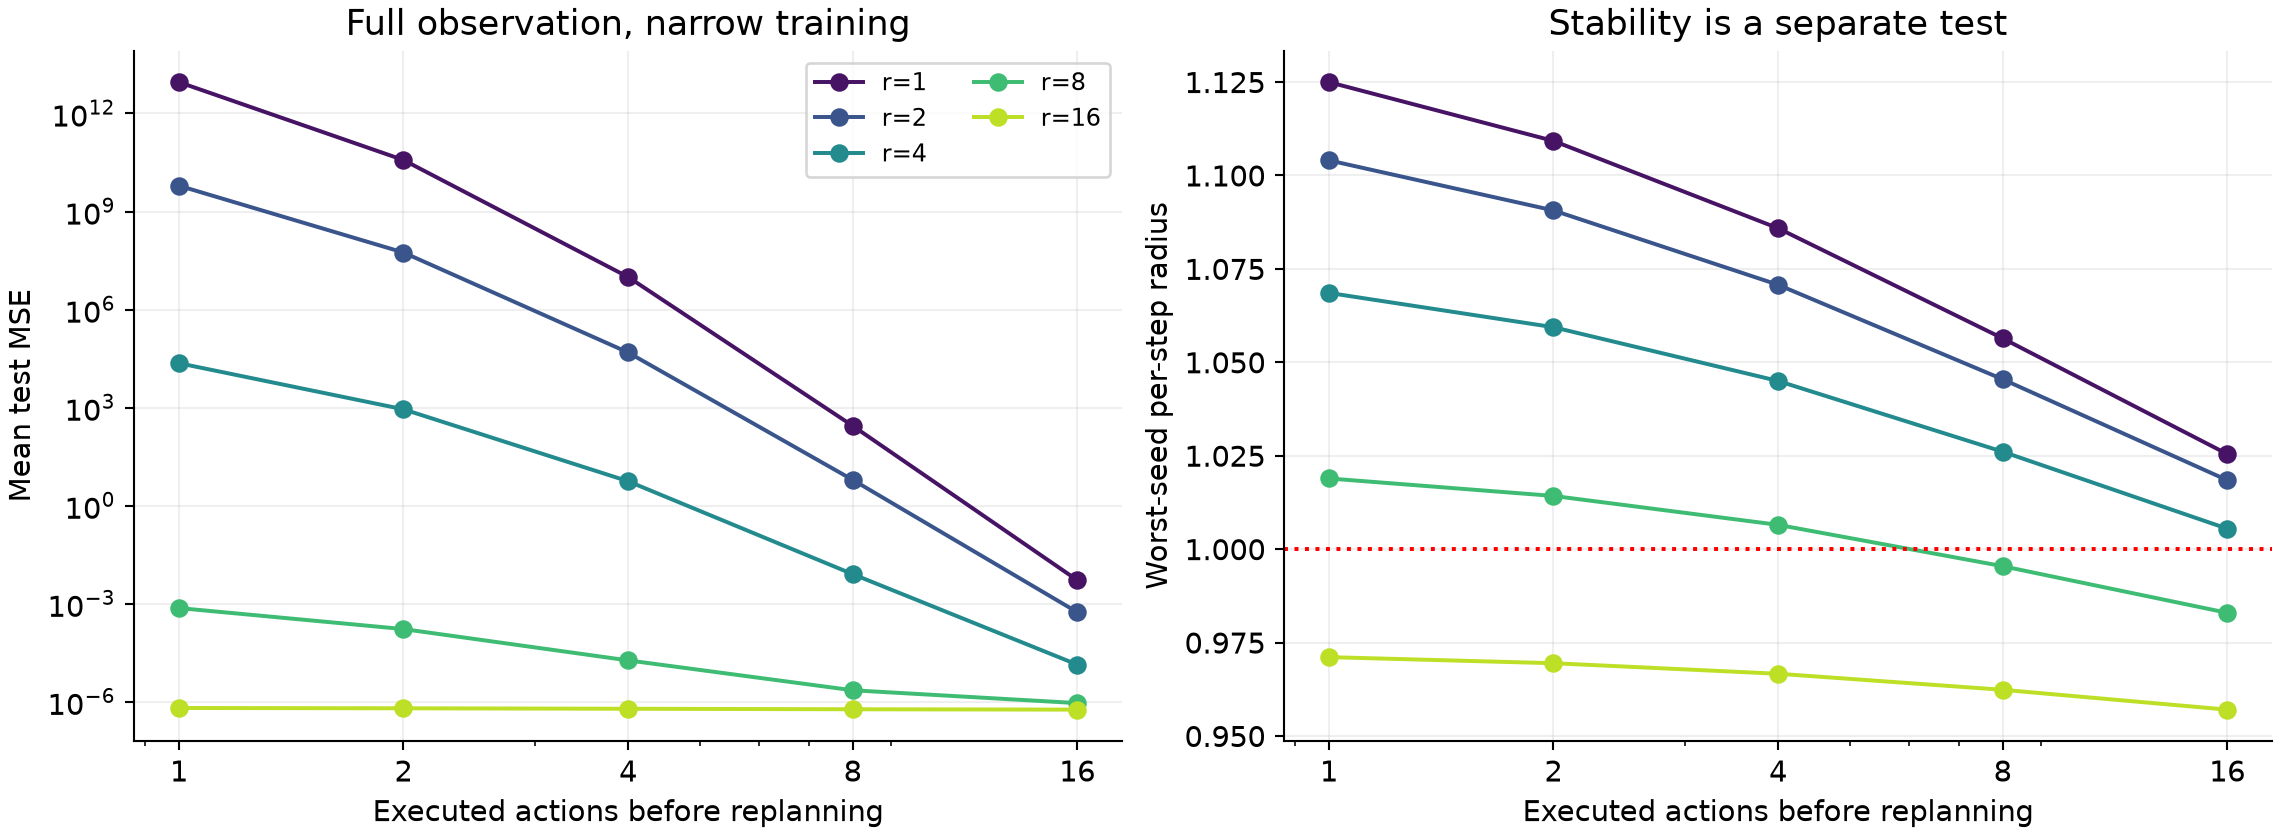
\includegraphics[width=\linewidth]{figures/history_execution.png}
\caption{Full-observation narrow-data sweep at H=16. Left: mean test MSE over five training seeds. Right: worst-seed per-step spectral radius. The red line marks the stability boundary.}
\end{figure}

{\small\setlength{\tabcolsep}{3pt}
\begin{longtable}{@{}p{\dimexpr 0.12311\linewidth-2\tabcolsep\relax}p{\dimexpr 0.30303\linewidth-2\tabcolsep\relax}p{\dimexpr 0.18939\linewidth-2\tabcolsep\relax}p{\dimexpr 0.38447\linewidth-2\tabcolsep\relax}@{}}
\toprule
\textbf{History} & \textbf{Mean MSE at $\ell$=1} & \textbf{Worst rate} & \textbf{Shortest passing execution} \\
\midrule\endfirsthead
\toprule
\textbf{History} & \textbf{Mean MSE at $\ell$=1} & \textbf{Worst rate} & \textbf{Shortest passing execution} \\
\midrule\endhead
\bottomrule\endfoot
1 & $9.11\times10^{12}$ & 1.12498 & None \\
2 & $6.18\times10^{9}$ & 1.10405 & None \\
4 & $2.29\times10^{4}$ & 1.06857 & None \\
8 & 0.00074 & 1.01892 & 8 \\
16 & $6.49\times10^{-7}$ & 0.97110 & 1 \\
\end{longtable}}

At history eight, executing one action remains unstable (rate 1.01892), whereas execution eight is stable (0.99544) and has mean test MSE $2.26\times10^{-6}$. At history sixteen, execution one is stable (0.97110) with mean MSE $6.49\times10^{-7}$. This supports a reduction in the need for commitment within this grid.

A setting passes only if every seed is stable and its mean perturbed-test MSE is at most $1\times10^{-5}$. The threshold is illustrative, not a paper-prescribed target. None means no tested setting passes. History sixteen already observes the same full state as history one; its benefit is not extra sensing information.

{\small Source: \path{pitfalls/results/context_chunking/metrics.csv} and \path{context_summary.csv}. Curves use H=16 and arithmetic means across five seeds.\par}

\section{Sensing versus coverage: the four-way comparison}
Each sensing/training condition contains 135 learned records across three seeds, histories 1,2,4,8,16, prediction lengths 1,4,16 and valid execution prefixes. Each controller uses the same 40 held-out states. The comparison below fixes one-step execution and H=16.

\begin{figure}[htbp]\centering
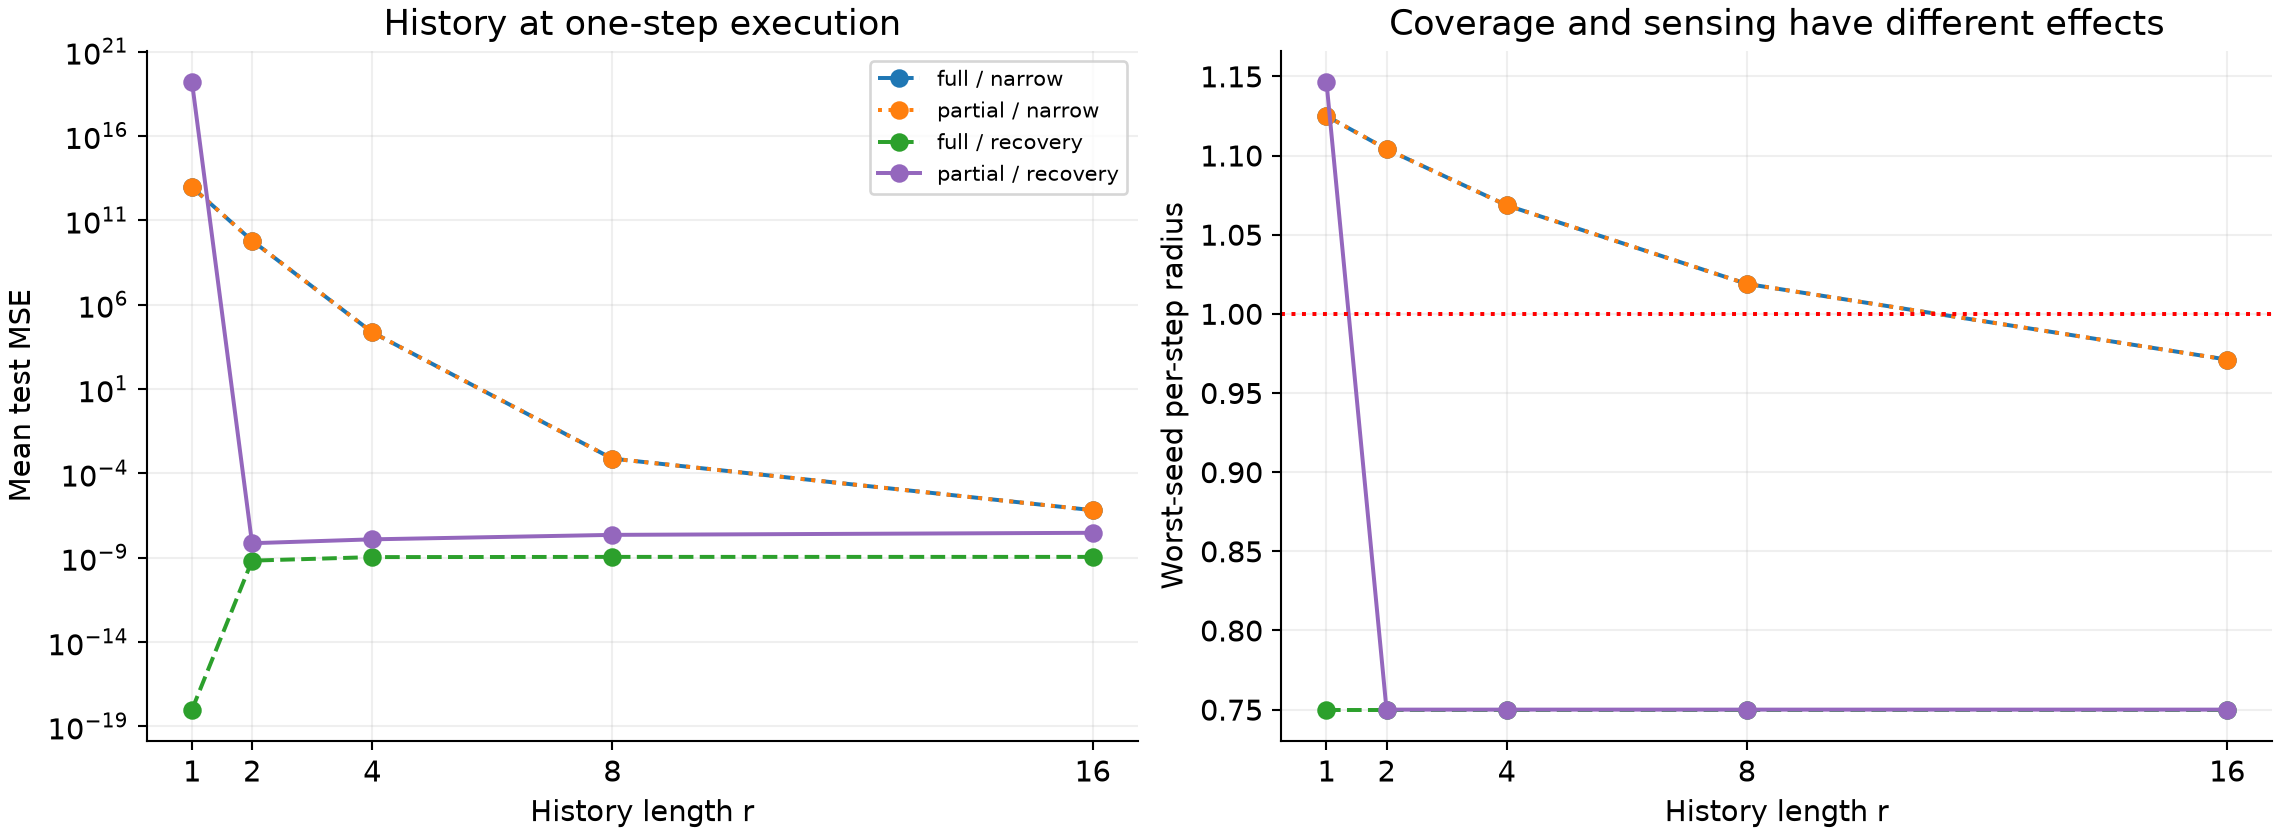
\includegraphics[width=\linewidth]{figures/coverage_sensing.png}
\caption{Matched full/partial sensing and narrow/recovery training at one-step execution, H=16. Scores are arithmetic means across three training seeds; the stability panel reports worst-seed rates.}
\end{figure}

{\small\setlength{\tabcolsep}{3pt}
\begin{longtable}{@{}p{\dimexpr 0.28788\linewidth-2\tabcolsep\relax}p{\dimexpr 0.09848\linewidth-2\tabcolsep\relax}p{\dimexpr 0.24621\linewidth-2\tabcolsep\relax}p{\dimexpr 0.19318\linewidth-2\tabcolsep\relax}p{\dimexpr 0.17424\linewidth-2\tabcolsep\relax}@{}}
\toprule
\textbf{Condition} & \textbf{History} & \textbf{Mean test MSE} & \textbf{Worst rate} & \textbf{Stable seeds} \\
\midrule\endfirsthead
\toprule
\textbf{Condition} & \textbf{History} & \textbf{Mean test MSE} & \textbf{Worst rate} & \textbf{Stable seeds} \\
\midrule\endhead
\bottomrule\endfoot
full / narrow & 2 & $6.18\times10^{9}$ & 1.10405 & 0/3 \\
partial / narrow & 2 & $6.18\times10^{9}$ & 1.10405 & 0/3 \\
partial / narrow & 16 & $6.49\times10^{-7}$ & 0.97110 & 3/3 \\
full / recovery & 1 & $9.78\times10^{-19}$ & 0.75000 & 3/3 \\
partial / recovery & 1 & $1.54\times10^{19}$ & 1.14636 & 0/3 \\
partial / recovery & 2 & $7.15\times10^{-9}$ & 0.75000 & 3/3 \\
partial / recovery & 16 & $2.97\times10^{-8}$ & 0.75000 & 3/3 \\
\end{longtable}}

Two results separate the mechanisms. First, full and partial narrow fits coincide across all paired settings: omitting an always-zero training feature does not change the effective ridge fit. Second, recovery training works with history one under full sensing but needs history two under partial sensing. Better coverage cannot compensate for insufficient current information in the tested history-one learner.

{\small The saved on-support controls sharpen this interpretation. Partial recovery at r=1 already has mean MSE $1.53\times10^{19}$ when $x_1$ starts at zero, almost the same as its perturbed loss. It fails nominal tracking too, not only hidden-jump recovery. At r=2, support MSE is $6.82\times10^{-15}$ while perturbed MSE is $7.15\times10^{-9}$, isolating the remaining recovery transient.\par}

{\small More data do not uniformly help: partial recovery at history one is worse than partial narrow and remains unstable. The added examples cannot be represented accurately from a single scalar observation. These statements concern this learner and protocol, not all partial-observation controllers.\par}

\section{How execution changes the result}
Execution length is the number of predicted actions committed before using new observations to replan. It differs from prediction length: H says how many actions are predicted, while $\ell$ says how many of them are actually used.

{\small\setlength{\tabcolsep}{3pt}
\begin{longtable}{@{}p{\dimexpr 0.19886\linewidth-2\tabcolsep\relax}p{\dimexpr 0.39962\linewidth-2\tabcolsep\relax}p{\dimexpr 0.40152\linewidth-2\tabcolsep\relax}@{}}
\toprule
\textbf{Executed prefix} & \textbf{Partial narrow, r=8\newline Mean MSE / rate} & \textbf{Partial recovery, r=2\newline Mean MSE / rate} \\
\midrule\endfirsthead
\toprule
\textbf{Executed prefix} & \textbf{Partial narrow, r=8\newline Mean MSE / rate} & \textbf{Partial recovery, r=2\newline Mean MSE / rate} \\
\midrule\endhead
\bottomrule\endfoot
1 & 0.00074 / 1.01892 & $7.15\times10^{-9}$ / 0.75000 \\
2 & 0.000168 / 1.01424 & $1.65\times10^{-8}$ / 0.75000 \\
4 & $1.85\times10^{-5}$ / 1.00651 & $4.11\times10^{-8}$ / 0.75000 \\
8 & $2.26\times10^{-6}$ / 0.99544 & $1.08\times10^{-7}$ / 0.75000 \\
16 & $9.15\times10^{-7}$ / 0.98296 & $2.64\times10^{-7}$ / 0.75001 \\
\end{longtable}}

\paragraph{Commitment helps a bad feedback extension}
For narrow training at r=8, longer execution reduces the measured loss and eventually stabilizes the fitted controller. It postpones repeated use of a feedback rule that is inaccurate on off-demonstration histories. Execution eight is the shortest tested setting passing the stated criterion.

\paragraph{Commitment delays correction once learning succeeds}
For partial recovery at r=2, all listed execution lengths are stable, but error rises from $7.15\times10^{-9}$ at $\ell$=1 to $2.64\times10^{-7}$ at $\ell$=16, about 37 times larger. The initial departure becomes observable after one transition; a committed controller cannot revise actions until the next boundary. Thus the delayed-feedback cost appears even without continuing noise.

\paragraph{Predicting farther ahead has no independent effect here}
Ridge regression fits output columns independently. With matched inputs, adding future-action targets leaves the earlier fitted action rows unchanged. All saved sweeps satisfy prefix agreement to numerical precision (maximum relative loss gap about $4.2\times10^{-9}$). Overlapping H curves are a property of this model, not evidence that chunk training never matters for shared-parameter neural learners.

{\small Across both narrow sensing conditions, shortest passing execution is None, None, None, 8, 1 as history grows. For full recovery, it is 1 at every history. For partial recovery it is None at history one, then 1 at every tested history of at least two.\par}

\section{What the partial-observation learner actually sees}
The partial sensor is y=$x_2$. Its two-observation matrix has rows [0,1] and [-0.1875,0.75], with nonzero determinant. The noiseless plant is observable with history two. This is a statement about available information, not a guarantee that a learner uses it.

\begin{figure}[htbp]\centering
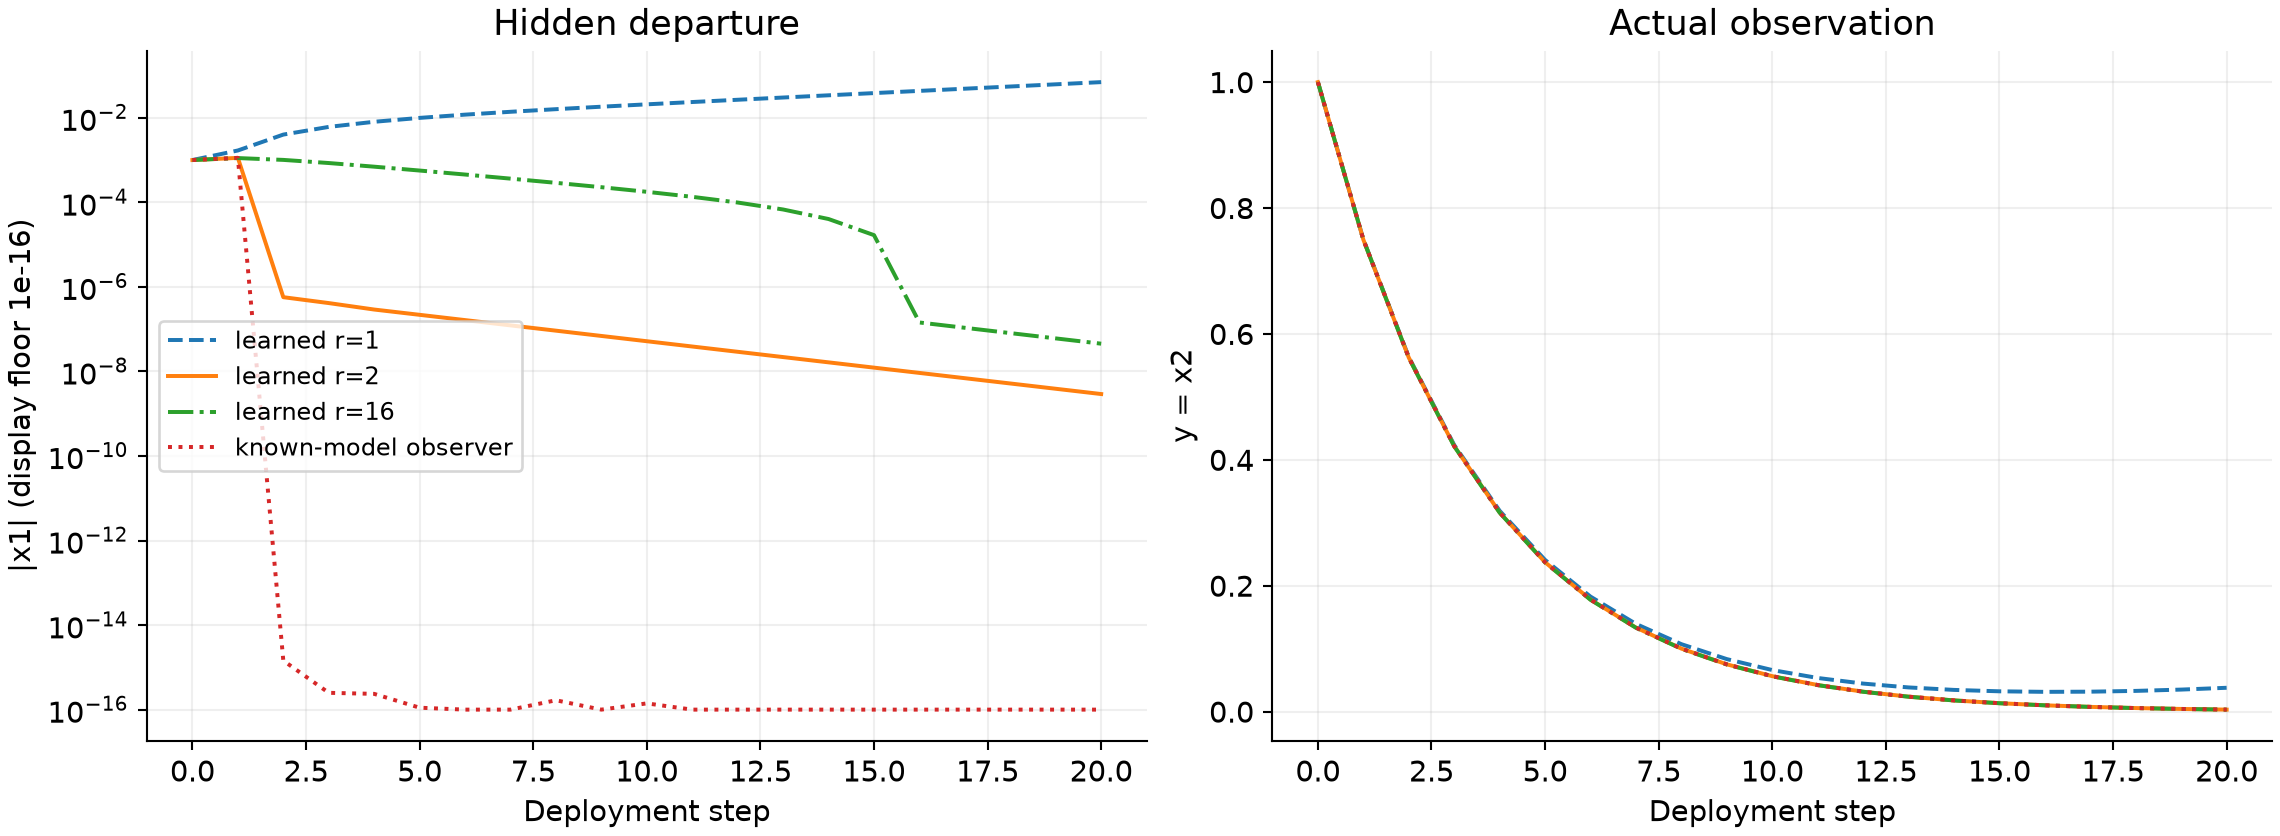
\includegraphics[width=\linewidth]{figures/learner_early.png}
\caption{First 20 steps of the canonical partial-recovery rollout, seed 618, H=16 and one-step execution. State departure is hidden from the learner; only the right panel is directly observed. Display floor: $1\times10^{-16}$.}
\end{figure}

{\small\setlength{\tabcolsep}{3pt}
\begin{longtable}{@{}p{\dimexpr 0.08523\linewidth-2\tabcolsep\relax}p{\dimexpr 0.20833\linewidth-2\tabcolsep\relax}p{\dimexpr 0.21780\linewidth-2\tabcolsep\relax}p{\dimexpr 0.26515\linewidth-2\tabcolsep\relax}p{\dimexpr 0.22348\linewidth-2\tabcolsep\relax}@{}}
\toprule
\textbf{Step} & \textbf{Hidden $x_1$} & \textbf{Observed $x_2$} & \textbf{Model estimate $x_1$} & \textbf{Applied u1} \\
\midrule\endfirsthead
\toprule
\textbf{Step} & \textbf{Hidden $x_1$} & \textbf{Observed $x_2$} & \textbf{Model estimate $x_1$} & \textbf{Applied u1} \\
\midrule\endhead
\bottomrule\endfoot
0 & 0.001 & 1.0000000 & 0 & -0.1874993 \\
1 & 0.00113 & 0.7498124 & 0.00113 & -0.1418557 \\
2 & $5.7\times10^{-7}$ & 0.5623592 & $5.7\times10^{-7}$ & -0.1054426 \\
\end{longtable}}

At the first decision, perturbed and unperturbed states have identical partial-observation features. The history-two learner therefore cannot immediately condition its action on the hidden jump. At the next step, the changed $x_2$ and known preceding action reveal $x_1$. The displayed known-model estimate is a diagnostic; learned policies are not given this reconstructed state.

In the saved canonical recovery trace, |$x_1$| first drops below $1\times10^{-6}$ at steps 2,4,8,16 for learned histories 2,4,8,16, respectively. The model observer reaches that level at step 2. Longer buffers retain more of the initialization mismatch; this is consistent with the slower correction visible in the traces. It is not a proof that every longer history must be slower.

{\small The complete learner\_view.png also plots reconstruction and action errors. On unstable trajectories, absolute floating-point reconstruction error can grow with state magnitude even when the reconstruction identity remains valid mathematically. The $1\times10^{-16}$ trace floor is display-only.\par}

\section{Mean loss, seed variation and reference controllers}
For each trained controller, test MSE averages ||x\_learner - x\_expert|| squared over the 20 perturbed states and 200 scored steps. The arithmetic mean across training seeds estimates expected loss over training and test randomness. The expert Kx is deterministic; exploration and sampled states supply randomness. Coordinates receive equal weight, with no per-coordinate normalization.

{\small\setlength{\tabcolsep}{3pt}
\begin{longtable}{@{}p{\dimexpr 0.47917\linewidth-2\tabcolsep\relax}p{\dimexpr 0.28409\linewidth-2\tabcolsep\relax}p{\dimexpr 0.23674\linewidth-2\tabcolsep\relax}@{}}
\toprule
\textbf{Partial recovery, r=1, $\ell$=1} & \textbf{Test MSE} & \textbf{Per-step rate} \\
\midrule\endfirsthead
\toprule
\textbf{Partial recovery, r=1, $\ell$=1} & \textbf{Test MSE} & \textbf{Per-step rate} \\
\midrule\endhead
\bottomrule\endfoot
Training seed 618 & $2.38\times10^{14}$ & 1.12640 \\
Training seed 619 & $9.38\times10^{12}$ & 1.12491 \\
Training seed 620 & $4.61\times10^{19}$ & 1.14636 \\
Mean across seeds & $1.54\times10^{19}$ & - \\
Median across seeds & $2.38\times10^{14}$ & - \\
\end{longtable}}

The largest seed contributes more than 99.99\% of the total loss in this setting. The mean $1.54\times10^{19}$ and median $2.38\times10^{14}$ answer different questions. Reporting the mean exposes catastrophic fits; reporting only the median would obscure their expected-cost impact. Three seeds are inadequate for a precise tail-risk or confidence claim.

{\small\setlength{\tabcolsep}{3pt}
\begin{longtable}{@{}p{\dimexpr 0.46402\linewidth-2\tabcolsep\relax}p{\dimexpr 0.18939\linewidth-2\tabcolsep\relax}p{\dimexpr 0.34659\linewidth-2\tabcolsep\relax}@{}}
\toprule
\textbf{Reference on the current test set} & \textbf{Mean MSE} & \textbf{Information used} \\
\midrule\endfirsthead
\toprule
\textbf{Reference on the current test set} & \textbf{Mean MSE} & \textbf{Information used} \\
\midrule\endhead
\bottomrule\endfoot
expert K1 & 0 & Full-state expert \\
analytic memory (model-informed) & $1.74\times10^{-8}$ & Full-state + known model \\
zero control (stable plant reference) & 0.0822 & No observations \\
known-model observer (partial) & $7.15\times10^{-9}$ & Partial histories + known model \\
\end{longtable}}

The partial recovery learner at r=2 has mean MSE $7.15418\times10^{-9}$, nearly matching the partial model observer at $7.15412\times10^{-9}$. This demonstrates successful learning of useful history-based behavior under informative coverage. It does not establish the observer as the optimal possible tracking policy. Full-state references have privileged information under partial sensing.

{\small Averages can also hide difficult test states: for partial recovery r=2, the worst saved perturbed-rollout MSE is $1.44\times10^{-8}$, about twice the mean. The pass rule constrains each seed mean; it does not require every individual test rollout to satisfy the threshold.\par}

{\small Original charts generally show medians across seeds; this report recomputes means from raw rows. Finite-horizon loss depends on time, units and perturbation scale. Without continuing noise, stable transient errors can average toward zero as the horizon grows, even for imperfect tracking.\par}

\section{Stability, long runs and the theory connection}
The exact boundary map includes the plant state and history buffers, with actions frozen within each chunk. Spectral radius below one establishes asymptotic stability for this linear controller. Compare radius\textasciicircum{}(1/$\ell$) across execution lengths; the raw boundary radius covers different durations.

{\small\setlength{\tabcolsep}{3pt}
\begin{longtable}{@{}p{\dimexpr 0.24621\linewidth-2\tabcolsep\relax}p{\dimexpr 0.26326\linewidth-2\tabcolsep\relax}p{\dimexpr 0.27462\linewidth-2\tabcolsep\relax}p{\dimexpr 0.21591\linewidth-2\tabcolsep\relax}@{}}
\toprule
\textbf{History / execution} & \textbf{200-step test-set mean} & \textbf{1000-step canonical mean} & \textbf{Worst rate} \\
\midrule\endfirsthead
\toprule
\textbf{History / execution} & \textbf{200-step test-set mean} & \textbf{1000-step canonical mean} & \textbf{Worst rate} \\
\midrule\endhead
\bottomrule\endfoot
r=4, $\ell$=16 & $1.38\times10^{-5}$ & 0.0191 & 1.00548 \\
r=8, $\ell$=1 & 0.00074 & $1.47\times10^{9}$ & 1.01892 \\
r=8, $\ell$=8 & $2.26\times10^{-6}$ & $5.12\times10^{-7}$ & 0.99544 \\
r=16, $\ell$=1 & $6.49\times10^{-7}$ & $1.22\times10^{-7}$ & 0.97110 \\
\end{longtable}}

The columns use different initial-state collections and horizons; they are not a paired estimate of horizon effects. Nonetheless the unstable r=8,$\ell$=1 controller has an enormous long-run canonical error despite modest 200-step test loss. Even r=4,$\ell$=16 remains unstable at rate 1.00548, so its small short-run error cannot justify deployment.

\paragraph{What Kyle's theory supports}
Reconstruction explains why history two can contain enough information under partial observation. His chunk-stability proposition explains suppression of feedback sensitivity through commitment, subject to decaying incremental plant responses and chunk sensitivities. It does not itself prove that more history shortens execution: its constants become more conservative with context, and it assumes $\ell$ at least r-1.

\paragraph{What is separately derived for this ridge example}
Narrow histories are rank one. Their closed-form ridge fit distributes feedback over past observations and actions. A small-gain certificate for one-step control is 48 $\alpha_r$ + $\beta_r$ \textless{} 1, where $\alpha_r$ and $\beta_r$ are absolute coefficient sums. In the zero-penalty limit its value is 1.8536 at r=8 and 0.2021 at r=16, certifying the latter. This is learner- and plant-specific; it is a stability certificate, not a monotone MSE theorem.

Neither reconstruction nor the chunk theorem identifies an expert from uncovered training directions. A broader learner theorem still needs deployment-error or gain guarantees. The experiments do not verify every policy-class assumption in Kyle's chunk bound and should not be presented as a direct numerical validation of that bound.

\section{Archived runs: what changes, and what survives}
Archived results are retained evidence, not discarded failures. Their protocols differ from the active recovery tests; they cannot be pooled into one performance estimate.

{\small\setlength{\tabcolsep}{3pt}
\begin{longtable}{@{}p{\dimexpr 0.22538\linewidth-2\tabcolsep\relax}p{\dimexpr 0.31629\linewidth-2\tabcolsep\relax}p{\dimexpr 0.11364\linewidth-2\tabcolsep\relax}p{\dimexpr 0.34470\linewidth-2\tabcolsep\relax}@{}}
\toprule
\textbf{Saved run} & \textbf{Protocol} & \textbf{Learned rows} & \textbf{Main finding} \\
\midrule\endfirsthead
\toprule
\textbf{Saved run} & \textbf{Protocol} & \textbf{Learned rows} & \textbf{Main finding} \\
\midrule\endhead
\bottomrule\endfoot
aligned & 200 steps; continuing noise SD .01; H=16; $r\leq8$ & 900 & Full persistent excitation succeeds; partial persistent excitation fails. \\
chunk\_execution & 200 steps; continuing noise; fixed r=2; varied H and $\ell$ & 450 & H prefixes overlap; execution changes feedback. \\
hard\_chunk\_execution & 60-step noiseless recovery; $r\leq8$ & 300 & Longer history/commitment lowers loss, but finite loss does not replace stability. \\
\end{longtable}}

{\small\setlength{\tabcolsep}{3pt}
\begin{longtable}{@{}p{\dimexpr 0.43561\linewidth-2\tabcolsep\relax}p{\dimexpr 0.08523\linewidth-2\tabcolsep\relax}p{\dimexpr 0.26515\linewidth-2\tabcolsep\relax}p{\dimexpr 0.21402\linewidth-2\tabcolsep\relax}@{}}
\toprule
\textbf{Noisy aligned condition ($\ell$=1)} & \textbf{r} & \textbf{Mean tracking MSE} & \textbf{Worst rate} \\
\midrule\endfirsthead
\toprule
\textbf{Noisy aligned condition ($\ell$=1)} & \textbf{r} & \textbf{Mean tracking MSE} & \textbf{Worst rate} \\
\midrule\endhead
\bottomrule\endfoot
full / initial & 1 & $2.43\times10^{-17}$ & 0.75000 \\
full / initial & 2 & $4.52\times10^{13}$ & 1.11191 \\
full / persistent & 2 & $1.05\times10^{-17}$ & 0.75000 \\
partial / persistent & 2 & $1.6\times10^{17}$ & 1.13782 \\
full / narrow & 8 & 2.92 & 1.01892 \\
\end{longtable}}

The initial-excitation regime illustrates a counterexample to universal history improvement: full observation succeeds at r=1 and fails at r=2. The expert immediately removes $x_1$, so later expert histories again have little coverage of recovery. Persistent process disturbances preserve coverage under full sensing but make current hidden state partly unpredictable under partial sensing.

{\small Current recovery data instead use known exploratory actions and noiseless state transitions, plus nominal expert continuation labels. Therefore the successful partial-recovery result is not a replication or refutation of the older noisy partial failure. Older chunk targets also include future noisy expert responses, unlike the current counterfactual labels. The earlier no-feasible-narrow result covered $r\leq8$, a different tolerance (RMS .05), and continuing noise.\par}

{\small The archived hard-example figure independently shows an initial $x_1$=0.001 growing to 1.17 under minimum-norm feedback and $1.80\times10^{16}$ under the wrong expert after 60 steps; the correct expert removes it. Those static-controller curves illustrate the construction, not learned-policy performance.\par}

\section{How to use the outputs, and what to test next}
{\small\setlength{\tabcolsep}{3pt}
\begin{longtable}{@{}p{\dimexpr 0.44508\linewidth-2\tabcolsep\relax}p{\dimexpr 0.55492\linewidth-2\tabcolsep\relax}@{}}
\toprule
\textbf{Output} & \textbf{Question it answers} \\
\midrule\endfirsthead
\toprule
\textbf{Output} & \textbf{Question it answers} \\
\midrule\endhead
\bottomrule\endfoot
metrics.csv & How does each trained controller perform, and is its fitted loop stable? \\
test\_rollouts.csv / test\_states.csv & Which individual test cases produce the aggregate loss? \\
context\_summary.csv / execution\_candidates.csv & Which tested execution lengths pass every-seed loss and stability checks? \\
sample\_trajectories.csv / sample\_rollouts.png & How does one fixed deployment evolve? These are not test-set averages. \\
learner\_inputs.csv / learner\_view.csv & What observations and actions enter the partial policy, and what does it do? \\
baselines.csv & How do expert, zero, analytic-memory and observer references compare? \\
config.json / source\_manifest.json & Which protocol and exact saved files underpin the conclusions? \\
\end{longtable}}

\paragraph{Main limitations}
The fixed plant is open-loop stable; the test departures are small and drawn from a narrow chosen range. Initialization relies on expert warm-up. Current tests have no continuing process or measurement noise. Recovery training assumes state-aware expert labels and a simulator to form future expert targets. Three or five reused seeds do not justify statistical confidence or a generalization theorem. Thresholds and investigated history grids were explored on these data; confirmation needs fresh data.

\paragraph{Next experiments, in order}
1. Freeze a meaningful loss/stability criterion, then repeat with fresh training and test seeds. Report seed means, ranges and instability counts.\\
2. Sweep perturbation magnitude and test horizon. Compare cumulative and late-window errors as well as full-episode MSE, so transient dilution cannot drive the conclusion.\\
3. Add measurement and process noise separately. Compare raw-history learning against an observer with a stated noise model.\\
4. Check feature normalization and ridge penalties. Then vary plant stability and observability before extending to more general learners.

\paragraph{Source and reproduction notes}
{\small Active data: \path{pitfalls/results/context_chunking} and four suites under \path{pitfalls/results/partial_observation}: full narrow, partial narrow, full recovery, and partial recovery. Historical data: three suites under \path{archive/pitfalls-before-focus/results}: aligned, chunk execution, and hard chunk execution. Scalar-controller and optimization scripts in that archive have no additional retained result folders in this review; they are not extra empirical evidence. The separate cyclic observability study is outside this report's scope.\par}

\paragraph{Literature.} The construction and intervention rationale draw on \citet{simchowitz2025,laskey2017,ross2011,zhang2025}; these sources motivate mechanisms, not the exact sizes or protocols used here.


\clearpage
\begin{thebibliography}{4}
\bibitem[Simchowitz et al.(2025)]{simchowitz2025}
M. Simchowitz, D. Pfrommer, and A. Jadbabaie.
The pitfalls of imitation learning when actions are continuous.
\emph{arXiv:2503.09722v4}, 2025.
\bibitem[Laskey et al.(2017)]{laskey2017}
M. Laskey, J. Lee, R. Fox, A. Dragan, and K. Goldberg.
DART: Noise injection for robust imitation learning. \emph{CoRL}, 2017.
\bibitem[Ross et al.(2011)]{ross2011}
S. Ross, G. Gordon, and J.~A. Bagnell.
A reduction of imitation learning and structured prediction to no-regret online learning. \emph{AISTATS}, 2011.
\bibitem[Zhang et al.(2025)]{zhang2025}
T.~T. Zhang, D. Pfrommer, C. Pan, N. Matni, and M. Simchowitz.
Action chunking and exploratory data collection yield exponential improvements in behavior cloning for continuous control. \emph{arXiv:2507.09061v5}, 2025.
\end{thebibliography}
\end{document}
